\documentclass[a4paper]{article}

\usepackage[utf8]{inputenc}
\usepackage{graphicx}
\usepackage{mathtools}

\begin{document}
\title{Machine Learning - Exercise 1 }
\author{Deniz Kocabas and Hans-Jörg Schurr}

\maketitle
\tableofcontents
\newpage

\section{Introduction}
The Data Intensive Science has become an indispensable aspect of the people's lives. We use it in many different areas to gain knowledge by analysis of integrated data. The overall goal of that assignment is to perform experiments with regression techniques in machine learning. Regression is the easiest technique to use, but also the least powerful. There are a number of independent variables, which, when taken together, produce a result a dependent variable. The regression model is then used to predict the result of an unknown dependent variable, given the values of the independent variables. 

We had to pick three datasets from UCI Machine Learning Repository, which should have different characteristics. 
Our choice was:
\begin{enumerate}
    \item "Individual Household Electric Power Consumption Data Set" \\ (http://archive.ics.uci.edu/ml/datasets/Individual+household+electric+power+consumption)
    \item "Solar Flare Data Set" \\
        (http://archive.ics.uci.edu/ml/datasets/Solar+Flare)
    \item "Wine Quality Data Set" \\
        (http://archive.ics.uci.edu/ml/datasets/Wine+Quality)
\end{enumerate}

We have used 4 different regression techniques by the tool \emph{Weka}. 
These techniques were;
\begin{enumerate}
    \item Simple Linear Regression
    \item Linear Regression
    \item SMOReg
    \item M5P
\end{enumerate}

\section{The chosen datasets}
The household electric power consumption data set contains over two million
instances and is by far the largest dataset among those three sets. The dataset
has nine dimensions, whereby two fields are used for a time stamp. Thus it is a
timeseries. All other fields contain numeric data. According to the
documentation 1.25 percent of the rows contain missing values. We decided to use
this dataset to test the performance of the methods. Given the high number of
missing values, this dataset is suited to test different methods to handle those
missing values. This dataset contains 3 class labels, which are sub-metering No. 1, 
energy sub-metering No. 2,  energy sub-metering No. 3 represents the active energy 
consumed every minute in watt hour. No. 1 corresponds to the kitchen, containing mainly 
a dishwasher, an oven and a microwave (hot plates are not electric but gas powered). 
No. 2 corresponds to the laundry room, containing a washing-machine, a tumble-drier, 
a refrigerator and a light. And No. 3 corresponds to an electric water-heater and an air-conditioner. 

The solar flare data set is with roughly 1400 instances much smaller then the
household electric power consumption data set. Every instance has ten fields,
which contain mainly categorical data. Some of those map to numeric intervals
(area of the spots). The set lacks missing values, therefore it is well suited
to test various methods to handle categorical data. The database has 3 class labels, 
one for the number times a certain type of solar flare occured in a 24 hour period. 
These 3 class labels are C-class flares (common flares), M-class flares (moderate flares), 
X-class flares (severe flares) production by this region in the following 24 hours. 
Each instance represents captured features for 1 active region on the sun. 
There are 2 files and the second file has had much more error correction applied to the it, 
and has consequently been treated as more reliable. 

We decided to choose a set with medium size and mixed features as third set. The
wine quality data set provided those requirements. It contains around 5000
instances and no missing values. The twelve attributes contain mainly numeric
values. Most of those are chemical properties of the wines. The last field is
the class value is based on sensory data, median of at least 3 evaluations made by wine experts. 
Each expert graded the wine quality  an assigned quality of the wine. It is natural number 
between one (very bad) and ten (very excellent).
Given the fact, that it is not exactly measured it may behave like a
categorical value. There are two dataset, one is for the red wine and the other for white wine.

\section{Methods tried}

The Simple Linear Regression techniques is the Linear Regression with one variable. The algorithm in \emph{Weka} picks the attribute with the lowest squared error. The algorithm can not deal with the missing values, so we need to preprocess before the algorithm and also just the numeric values should be in the attributes, otherwise \emph{Weka} can not use this algorithm. We should remove or preprocess these other types of dimensions. The hypothesis formula is;
\begin{equation*}
h_\theta (x) = \theta_0+ \theta_1 x_1
\end{equation*}

The Linear Regression techniques is for the multiple variable. The algorithm in \emph{Weka} uses the Akaike criterion. It is a measure of the relative quality of a statistical model, for a given set of data. As such, AIC provides a means for model selection. The algorithm is able to deal with weighted instances. The hypothesis formula is for the multi dimensional model;

\begin{equation*}
h_\theta (x) = \theta^T x =\theta_0 x_0+ \theta_1 x_1 + \dots + \theta_n x_n
\end{equation*}

     The algorithm SMOReg in \emph{Weka} is the support vector machine for regression. The parameters can be learned using various algorithms. The algorithm is selected by setting the RegOptimizer. This implementation globally replaces all missing values and transforms nominal attributes into binary ones. It also normalizes all attributes by default.

     M5 Prunning(M5P)  is a non-linear regression, which implements base routines for generating M5 Model trees and rules. A model tree is a tree, where each leaf has got one of these linear regression model. It is like a patch work of linear models.  

\section{Experiments and results for the individual datasets}

\subsection{The household electric power consumption data set}
The household electric power consumption data set has a huge instance, which has almost two million instances. First we convert the file to csv and try to upload it to \emph{Weka}. We had an error out of memory, so we have changed the maxheap value to 4gb. Then our data uploaded to the \emph{Weka} without problem. In this file, there are some missing values. From the preprocess section, there is a function, which is called Replacemissingvalues. This function replaces all missing values for nominal and numeric attributes in dataset with the modes and mean from the training data. In that dataset, there are also 2 nominal attributes and this nominal attributes consist of more than 1400 distinct values. In that reason, it is hard to calculate the linear regression model with them. So we have removed these nominal attributes and deal just with the numeric attributes. After have removed nominal attributes and run the Replacemissingvalues function, we have passed the section to classify of the \emph{Weka}. There are 3 class variable in that dataset, we calculate the regression model for the class energy sub-metering No. 3 corresponds to an electric water-heater and an air-conditioner.

We have used the 10 folds Cross-validation techniques to split the data for test and train. It divides the dataset into 10 part and each 10 samples is retained as the validation data for testing the model, and the remaining 9 samples are used as training data. The cross-validation process is then repeated 10 times, with each of the 10 samples used exactly once as the validation data. The 10 results from the folds then can be averaged to produce a single estimation.  

At first we have run the Simple Linear Regression techniques, which is the least powerful algorithm. It chooses the attribute Global$\_$active$\_$power, which hast the lowest squared error. Linear regression on Global$\_$active$\_$power model is: 
\begin{equation*}
    5.1 * \textnormal{Global\_active\_power} + 0.9
\end{equation*}

After that we have used the Linear Regression techniques for the multiple variables. The technique choose some of the attributes for the regression model. The model is:
\begin{align*}
\textnormal{Sub\_metering\_3} = &-6.2151 * \textnormal{Global\_reactive\_power} +\\
                       &-0.0334 * \textnormal{Voltage} +\\
                       &1.2213 * \textnormal{Global\_intensity} + 9.627 
\end{align*}

So the class attribute depends on these variables above. The Voltage and Global$\_$reactive$\_$power have a negative marks, that means, if we decrease these attributes, we have more Sub$\_$metering$\_$3. And for the positive weight, we need to increase the attribute Global$\_$intensity.

The 3. technique is the SMOReg, the support vector machine for regression. We had problems and most of the case we had out of memory error again. So, we have increased the maxheap to 6gb and used Percentage split to choose the training testing data split. Because it will run one time with this split instead of 10 times run with the 10 fold cross validation. So we have splitted data to 75\% for the training set and 25\% for the test set. But still we could not reach any model. The algorithm have taken more than 6 hours.

And the last one is the tree model, M5 Prunning(M5P). We have used again 10 folds cross validation technique for the test and training data. In that model we have many leaf of the trees, which has a different linear regression model. In the household electric power consumption dataset, the algorithm generate 3180 leaf, different linear regression. It is quiet hard to show all of them and also the tree is a bit complicated in that dataset.

\subsection{The solar flare data set}
The solar flare file contains 2 datase. We have chosen the smallest dataset, which has around 300 instances. ({\tt flare1.csv}) This file has the smallest instance in our datasets. First we convert the file into excel file and upload it to \emph{Weka}. In this file, there are no missing values. So we do not need anything to do for the missing values. In that dataset we have also some attributes are in nominativ type. And start the algorithms in the classify section of the \emph{Weka}. There are 3 class variable in that dataset, we calculate the regression model for the class X flares (severe flares) production by this region in the following 24 hours. So we remove other 2 class label from the preprocess section. We have also used the 10 folds Cross-validation techniques to split the data for test and train. 

At first we have run the Simple Linear Regression techniques, which is the least powerful algorithm. This technique can just deal with the Numeric attributes. For this reason, we deleted the nominativ dimension from the dataset, which are the first 3 fields. It chooses the attribute Historically-complex, which hast the lowest squared error. Linear regression on Historically-complex model is: 
\begin{equation*}
    0.05 * \textnormal{Historically-complex} - 0.04
\end{equation*}

After that we have used the Linear Regression techniques for the multiple variables. We added the nominativ attributes again to our dataset and run the algorihm. The technique choose some of the attributes for the regression model. The model is:
\begin{align*}
\textnormal{X-class flares} =& 0.0334 * \textnormal{(Code for class=H,D)} +\\
                             &0.1165 * \textnormal{(Code for spot distribution=C)} +\\
                             &0.0271 * \textnormal{Historically-complex} + (-0.038)
\end{align*}

So the X-class flares depends on these variables. We can see above that two nominativ attribute called "Code for class" and "Code for spot distribution" are in our linear regression model.

The 3. technique is the SMOReg, the support vector machine for regression. In that technique all of the attributes have used in the model. We can see from the below that for the nominativ attribute all possible values are also in the model. Some of them has a negative marks, which can increase the class value, when we decrease these attributes. And for the positive weight, we need to increase. The model is:
\begin{align*}
\textnormal{weights }& \textnormal{(not support vectors):}\\
& -       0.0001 * \textnormal{(normalized) Code for class=C}\\
& +       0.0002 * \textnormal{(normalized) Code for class=D}\\
& +       0.0002 * \textnormal{(normalized) Code for class=B}\\
& +       0      * \textnormal{(normalized) Code for class=F}\\
& +       0.0002 * \textnormal{(normalized) Code for class=H}\\
& -       0.0006 * \textnormal{(normalized) Code for class=E}\\
& -       0.0002 * \textnormal{(normalized) Code for largest spot size=S}\\
& +       0.0004 * \textnormal{(normalized) Code for largest spot size=A}\\
& -       0.0001 * \textnormal{(normalized) Code for largest spot size=K}\\
& +       0.0002 * \textnormal{(normalized) Code for largest spot size=R}\\
& +       0.0002 * \textnormal{(normalized) Code for largest spot size=X}\\
& -       0.0005 * \textnormal{(normalized) Code for largest spot size=H}\\
& +       0.0002 * \textnormal{(normalized) Code for spot distribution=O}\\
& -       0.0007 * \textnormal{(normalized) Code for spot distribution=I}\\
& +       0.0002 * \textnormal{(normalized) Code for spot distribution=X}\\
& +       0.0002 * \textnormal{(normalized) Code for spot distribution=C}\\
& -       0.0006 * \textnormal{(normalized) Activity}\\
& +       0.0003 * \textnormal{(normalized) Evolution}\\
& +       0.0003 * \textnormal{(normalized) Previous 24 hour flare activity code}\\
& +       0.001  * \textnormal{(normalized) Historically-complex}\\
& +       0      * \textnormal{(normalized) Did region become historically complex on this pass across the sun's disk}\\
& +       0.0002 * \textnormal{(normalized) Area}\\
& +       0.0004 * \textnormal{(normalized) Area of the largest spot}\\
& -       0.0007\\
\end{align*}

And the last one is the tree model, M5 Prunning(M5P). In that model we have many leaf of the trees, which has a different linear regression model. In solar flare file, the algorithm generate 2 leaf nodes.

\begin{figure}[ht!]
\centering
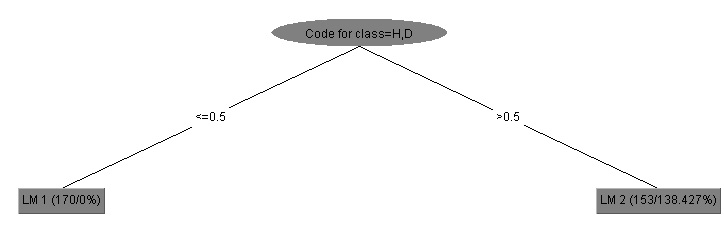
\includegraphics[width=120mm]{tree}
\caption{A simple caption}
\label{overflow}
\end{figure}

That means, there are 2 different linear regression model, which have shown in the below.\\
LM num: 1: 
\begin{align*}
    \textnormal{X-class flares} = &-0.0067 * \textnormal{(Code for class=H,D)}\\
                                  &+ 0.0093 *\textnormal{(Code for class=D)}\\ 
                                  &+ 0.0095 *\textnormal{(Code for spot distribution=X,C)} \\
                                  &+ 0.0022 *\textnormal{(Historically-complex)} - 0.0031\\
\end{align*}
LM num: 2:
\begin{align*}
    \textnormal{X-class flares}= &-0.0074 * \textnormal{(Code for class=H,D)} \\
                                 &+ 0.1174 *\textnormal{(Code for class=D)} \\
                                 &+ 0.1292 *\textnormal{(Code for spot distribution=X,C)} \\
                                 &+ 0.0552 *\textnormal{(Historically-complex)} - 0.1607\\
\end{align*}

\subsection{The wine quality data set}

The wine quality dataset contains 2 file, one is for the white wine and the other is red wine. We have chosen the white wine dataset, which has almost 5000 instances. First we convert the file to csv and upload it to \emph{Weka}. In this file, there are no missing values and all the attributes are real numbers. So we do not need any preprocess method. And start the algorithms in the clasify section of the \emph{Weka}. The class variable is quality attribute and its the number from one to ten. We have also used the 10 folds Cross-validation techniques to split the data for test and train. 

At first we have run the Simple Linear Regression techniques, which is the least powerful algorithm. It chooses the attribute alcohol, which hast the lowest squared error. Linear regression on alcohol model is: 
\begin{equation*}
    0.31 * \textnormal{alcohol} + 2.58
\end{equation*}

After that we have used the Linear Regression techniques for the multiple variables. The technique choose some of the attributes for the regression model. The model is:
\begin{align*}
    \textnormal{quality} = &0.0681 * \textnormal{fixed acidity} +\\
                           &-1.8881 * \textnormal{volatile acidity} +\\
                           & 0.0828 * \textnormal{residual sugar} +\\
                           & 0.0033 * \textnormal{free sulfur dioxide} +\\
                           &-154.2913 * \textnormal{density} +\\
                           &0.6942 * \textnormal{pH} +\\
                           &0.6285 * \textnormal{sulphates} +\\
                           &0.1932 * \textnormal{alcohol} + 154.1062\\
\end{align*}

So the quality depends on these variables above. Some of them has a negative marks, that means, if we decrease these attributes, we have better quality of wine. And for the positive weight, we need to increase.

The 3. technique is the SMOReg, the support vector machine for regression. In that technique all of the attributes have used in the linear regression model. The model is:
\begin{align*}
\textnormal{weights }& \textnormal{(not support vectors):} \\
& +       0.0754 * \textnormal{(normalized) fixed acidity}\\
& -       0.3535 * \textnormal{(normalized) volatile acidity}\\
& -       0.0291 * \textnormal{(normalized) citric acid}\\
& +       0.7259 * \textnormal{(normalized) residual sugar}\\
& -       0.0609 * \textnormal{(normalized) chlorides}\\
& +       0.2402 * \textnormal{(normalized) free sulfur dioxide}\\
& -       0.049  * \textnormal{(normalized) total sulfur dioxide}\\
& -       0.9238 * \textnormal{(normalized) density}\\
& +       0.1421 * \textnormal{(normalized) pH}\\
& +       0.1072 * \textnormal{(normalized) sulphates}\\
& +       0.2417 * \textnormal{(normalized) alcohol}\\
& +       0.3849\\
 \end{align*}

And the last one is the tree model, M5 Prunning(M5P). In that model we have many leaf of the trees, which has a different linear regression model. In the wine quality dataset, the algorithm generate 55 leaf, different linear regression. It is quiet hard to show all of them and also the tree is a bit complicated in that dataset.


\subsection{Comparison}

In that part, we wil describe and compare the error rate, coefficient corelation between the algorithms and also datasets each others. 

The correlation coefficient is a measure of linear association between two variables. Values of the correlation coefficient are always between -1 and +1. A correlation coefficient of +1 indicates that two variables are perfectly related in a positive linear sense, a correlation coefficient of -1 indicates that two variables are perfectly related in a negative linear sense, and a correlation coefficient of 0 indicates that there is no linear relationship between the two variable. For simple linear regression, the sample correlation coefficient is the square root of the coefficient of determination, with the sign of the correlation coefficient being the same as the sign of b1, the coefficient of x1 in the estimated regression equation.

The interpretation of these error in the table below are:

\begin{equation*}
    \textnormal{Mean absolute error} = \frac{|p_1 - a_1| + ... + |p_n - a_n|}{n}
\end{equation*}

\begin{equation*}
    \textnormal{Root mean squared error} =\sqrt{ \frac{(p_1 - a_1)^2 + ... + (p_n - a_n)^2}{n} }
\end{equation*}

When we compare the techniques, we have the biggest correlation coefficient from the model tree technique, m5p, which has many different linear regression model, and the time is also not that bad like SMOReg technique. In the largest dataset it took 5 minutes and for 2 million data, it was also not that much. The error rate is the lowest also in that regression technique. 

\begin{table}[b]
\begin{tabular}{| c | c | c |c |c |}
\hline & & & & \\
Technique & Time(s) & Correlation & Mean abs.  & Root mean \\
 & & coefficient & error & squared error  \\
\hline & & & &  \\
1  & 0.43  & 0.6386  & 5.0592  & 6.493  \\ 
\hline & & & & \\
2  & 8.64  & 0.6317  & 5.125  &  6.5403 \\ 
\hline & & & & \\
3  & $\ge$ 21600  & - & - & - \\ 
\hline & & & & \\
4  &  304.59 &  0.8506 & 2.3794 & 4.4367 \\ 
\hline
\end{tabular}
\caption{\textbf{Results of the Regression Techniques for the largest dataset, "Individual Household Electric Power Consumption Data Set" }}
    Algorithm 1: Simple Linear Regression,
    Algorithm 2: Linear Regression,
    Algorithm 3: SMOReg,
    Algorithm 4: M5P
\end{table}

The worst regression technique is the simplest one Simple Linear Regression, it uses just one attribute and has really bad results. It runs really fast, but we did not achieve a good result with it.

\begin{table}
\begin{tabular}{| c | c | c |c |c |c |}
\hline & & & & \\
Technique & Time(s) & Correlation & Mean abs.  & Root mean \\
 & & coefficient & error & squared error  \\
\hline & & & &  \\
1  & 0  & 0.0574  & 0.0425 & 0.146 \\ 
\hline & & & & \\
2  & 0.02  &  0.1028 & 0.0471 & 0.1469  \\ 
\hline & & & & \\
3  & 0.88  & -0.0092 & 0.0223 & 0.1472 \\ 
\hline & & & & \\
4  & 0.11  & 0.0625  & 0.046   & 0.1497 \\ 
\hline
\end{tabular}
\caption{\textbf{Results of the Regression Techniques for the smallest dataset,  "Solar Flare Data Set"}}
    Algorithm 1: Simple Linear Regression,
    Algorithm 2: Linear Regression,
    Algorithm 3: SMOReg,
    Algorithm 4: M5P
\end{table}

In the second dataset Solar Flare, in the result of the SMOReg, (Table 2) the correlation coefficient is really low, almost 0. It means, here is no linear relationship between the two variables. So that result is really bad, it is the smallest dataset and we can see from the result SMOReg have not good result for dataset with the small instance. And with that technique, we had many problems with the largest dataset. It took too much time to build a model with it, even with the percentage split technique. And finally we have needed to stop the technique. So we have no idea, how this techniques deal with the large data. 

\begin{table}
\begin{tabular}{| c | c | c |c |c |}
\hline & & & & \\
Technique & Time(s) & Correlation & Mean abs.  & Root mean \\
 & & coefficient & error & squared error  \\
\hline & & & &  \\
1  & 0.26   & 0.4345  & 0.628   &  0.7976\\ 
\hline & & & & \\
2  & 0.08  & 0.5257  & 0.5854 & 0.7534  \\ 
\hline & & & & \\
3  & 94.03  &  0.5225  & 0.5841 & 0.7564 \\ 
\hline & & & & \\
4  & 1.08  & 0.5866  & 0.5525  & 0.7188 \\ 
\hline
\end{tabular}
\caption{\textbf{Results of the Regression Techniques for the medium dataset, "Wine Quality Data Set"}}
    Algorithm 1: Simple Linear Regression,
    Algorithm 2: Linear Regression,
    Algorithm 3: SMOReg,
    Algorithm 4: M5P
\end{table}

The regular Linear Regression technique has a normal result, it has not bad result, but also not that good. This technique's results are always in the middle and the algorithm is quiet fast, when we compared with the other complicated ones.

In the 1. dataset, which is individual household electric power consumption, we had much problem to build the model, it took too much time with the SMOReg and M5P algorithms. But we had the best correlation coefficient in that dataset, which means two variables are perfectly related in a positive linear sense. But in the other way, we have the highest error rate. The minimum error rate was in the smallest instance dataset. The error rate was almost 0 in that data set Solar Flare dataset, and the process time is less then 1 second.


\section{Conclusion}

We have presented some of the regression techniques, with the different size of datasets. The regression problem is to predict a numeric value. We have used \emph{Weka} Explorer tool to compare these techniques and also the files. We had really good results with the largest dataset, although we had also some problems with it, when we were uploading the file into the \emph{Weka} and running the SMOReg algorithm in that dataset. SMOReg technique take much time, although we had not got a quiet nice result with it. The M5P regression technique was the best technique in our dataset. This technique is a tree model, where each leaf has got one of these linear regression model. It is like a patch work of linear models. The technique is also quiet fast and efficient. The regular technique's result is also sufficient. 

\end{document}
